\chapter{Background}
\section{Data Collection and Information Filtering}
\subsection{BigData}
The standards set by the World Wide Web consortium, formed in 1994, has led to large amounts of information sharing between the users and the hosts. As the users data grows, more hosts are required to sustain the growth. This growth can be viewed from the figure \autoref{fig:bigdata}.
\\
\begin{figure}[H]
	\centering
	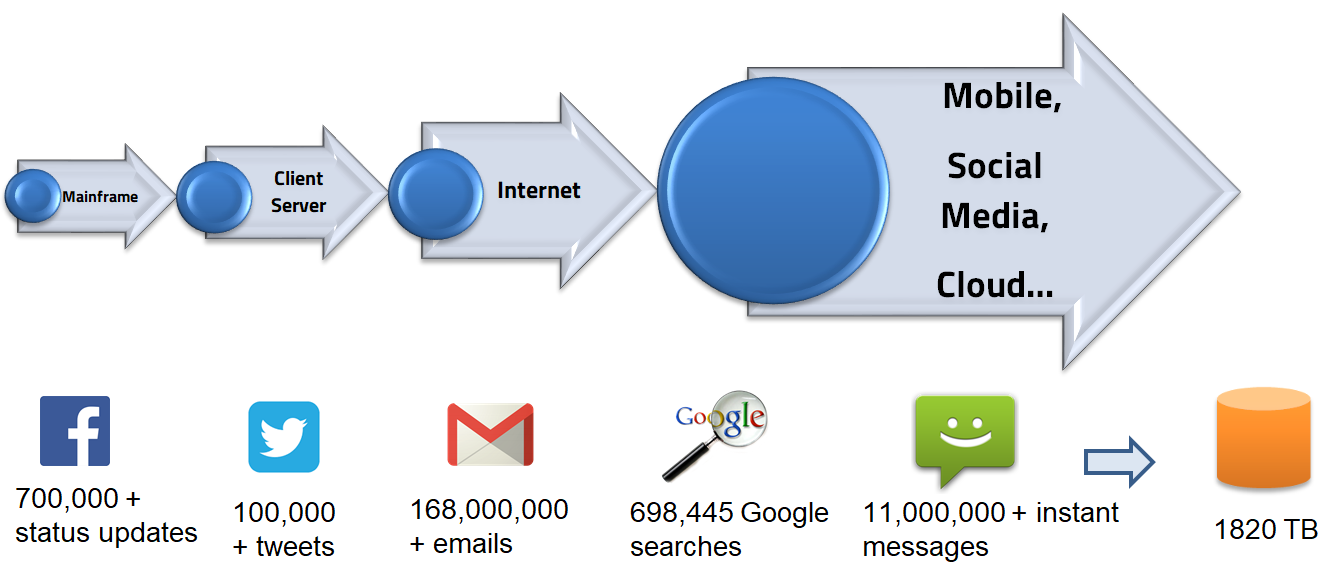
\includegraphics[width=0.7\linewidth]{bigdata}
	\caption{Growing Data Velocity per second}
	\label{fig:bigdata}
\end{figure}

\noindent To make any customer experience best, some of the ways recommendation technology is used to make it more personalize. These systems can perform well based on the more and more data. Bigdata is a driving force behind recommendation engines.
To make the this data useful, applications need to collect data filter data in specific patterns from which we will get useful information.

\subsection{Data Collection And Storage}

Information Gathering involves web crawling, document processing, indexing and queryprocessing. An architectural view of information gathering is shown in figure. A crawler processes all URLs via techniques like breadth-first search and depth-first search and stores the web servers response for each URL. The documents retrieved are then processed in order for its meta-data and to remove any noisy data. Data indexing is then applied so that retrieval and processing of extracted data is quicker.

\subsubsection{Implicit Data}
\subsubsection{Explicit Data}


\subsection{Information Filtering}

When a user requests information, it is treated as a query in the form of keywords and is applied on the indexed data. The objective of the query processor is to return most relevant documents to the user.

Filtering is a key component to retrieving adequate information per user preferences or user profile. User behavior is studied from past user profiles activities which helps to filter out any irrelevant data and provide apt suggestions pertaining to current needs. Part of information filtering that tries to predict a user's preference is known as a recommender system.